\documentclass[]{article}
\usepackage{lmodern}
\usepackage{amssymb,amsmath}
\usepackage{ifxetex,ifluatex}
\usepackage{fixltx2e} % provides \textsubscript
\ifnum 0\ifxetex 1\fi\ifluatex 1\fi=0 % if pdftex
  \usepackage[T1]{fontenc}
  \usepackage[utf8]{inputenc}
\else % if luatex or xelatex
  \ifxetex
    \usepackage{mathspec}
    \usepackage{xltxtra,xunicode}
  \else
    \usepackage{fontspec}
  \fi
  \defaultfontfeatures{Mapping=tex-text,Scale=MatchLowercase}
  \newcommand{\euro}{€}
\fi
% use upquote if available, for straight quotes in verbatim environments
\IfFileExists{upquote.sty}{\usepackage{upquote}}{}
% use microtype if available
\IfFileExists{microtype.sty}{%
\usepackage{microtype}
\UseMicrotypeSet[protrusion]{basicmath} % disable protrusion for tt fonts
}{}
\usepackage[margin=1in]{geometry}
\usepackage{longtable,booktabs}
\usepackage{graphicx}
\makeatletter
\def\maxwidth{\ifdim\Gin@nat@width>\linewidth\linewidth\else\Gin@nat@width\fi}
\def\maxheight{\ifdim\Gin@nat@height>\textheight\textheight\else\Gin@nat@height\fi}
\makeatother
% Scale images if necessary, so that they will not overflow the page
% margins by default, and it is still possible to overwrite the defaults
% using explicit options in \includegraphics[width, height, ...]{}
\setkeys{Gin}{width=\maxwidth,height=\maxheight,keepaspectratio}
\ifxetex
  \usepackage[setpagesize=false, % page size defined by xetex
              unicode=false, % unicode breaks when used with xetex
              xetex]{hyperref}
\else
  \usepackage[unicode=true]{hyperref}
\fi
\hypersetup{breaklinks=true,
            bookmarks=true,
            pdfauthor={JcB},
            pdftitle={Carte des RPU produits par territoire de santé},
            colorlinks=true,
            citecolor=blue,
            urlcolor=blue,
            linkcolor=magenta,
            pdfborder={0 0 0}}
\urlstyle{same}  % don't use monospace font for urls
\setlength{\parindent}{0pt}
\setlength{\parskip}{6pt plus 2pt minus 1pt}
\setlength{\emergencystretch}{3em}  % prevent overfull lines
\setcounter{secnumdepth}{0}

%%% Use protect on footnotes to avoid problems with footnotes in titles
\let\rmarkdownfootnote\footnote%
\def\footnote{\protect\rmarkdownfootnote}

%%% Change title format to be more compact
\usepackage{titling}

% Create subtitle command for use in maketitle
\newcommand{\subtitle}[1]{
  \posttitle{
    \begin{center}\large#1\end{center}
    }
}

\setlength{\droptitle}{-2em}
  \title{Carte des RPU produits par territoire de santé}
  \pretitle{\vspace{\droptitle}\centering\huge}
  \posttitle{\par}
  \author{JcB}
  \preauthor{\centering\large\emph}
  \postauthor{\par}
  \predate{\centering\large\emph}
  \postdate{\par}
  \date{08/01/2016}



\begin{document}

\maketitle


Objectif: dessiner une carte de l'Alsace avec une représentation du
nombre de RPU produits par chacun des douze territoires de proximié. Les
RPU sont représentés par des cercles dont la superficie est
proportionnelle au nombre de RPU.

Source: R et espace pp 189

Emplacement: RPU\_2014/Analyse/Carte\_RPU\_TP

Réalisation: il faut disposer:

\begin{itemize}
\itemsep1pt\parskip0pt\parsep0pt
\item
  d'un fond cartographique de l'Alsace: ctss
\item
  de la position des 12 villes correspondant au 12 territoires de
  proximité: ts
\item
  d'une liste du nombre de RPU par territoire de proximité
\end{itemize}

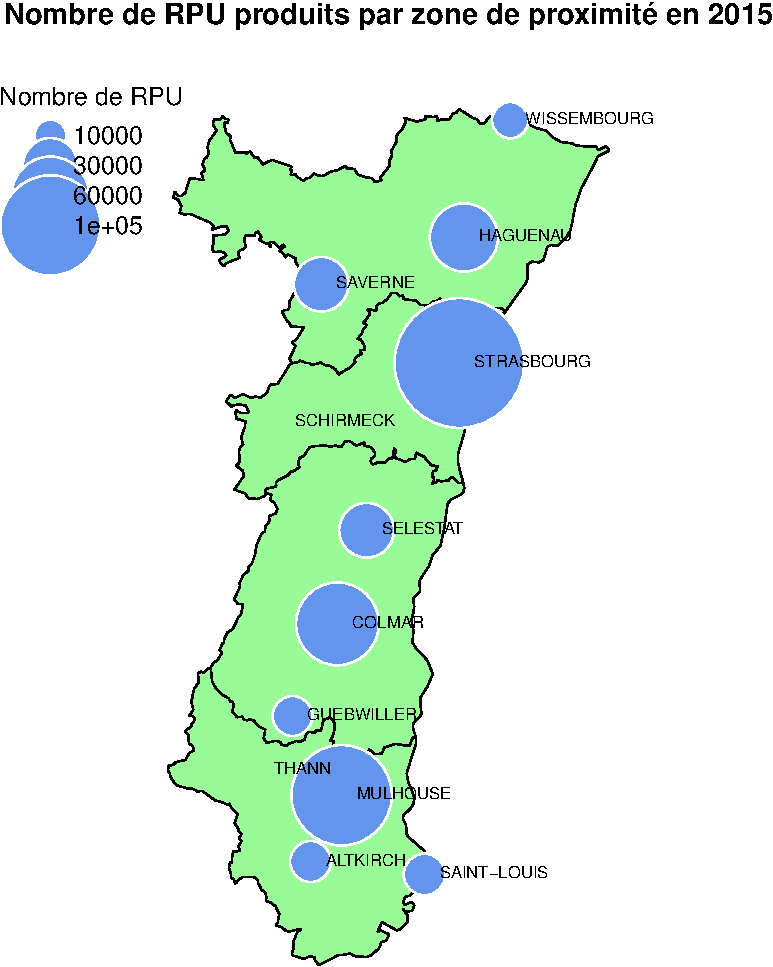
\includegraphics{carte_rpu_tp_files/figure-latex/carte-1.pdf}

La surface des cercles est proportionnelle au nombre de RPU. Il manque
des informations sur deux territoires: Schirmeck et Thann. En 2014, le
nombre de RPU de la zone Strasbourg est fortement sous estimé.

\begin{longtable}[c]{@{}llr@{}}
\caption{RPU produits en 2015 par zone de proximité}\tabularnewline
\toprule
& Zone de proximité & Nombre de RPU\tabularnewline
\midrule
\endfirsthead
\toprule
& Zone de proximité & Nombre de RPU\tabularnewline
\midrule
\endhead
27886 & ALTKIRCH & 16 831\tabularnewline
27940 & COLMAR & 68 231\tabularnewline
28053 & GUEBWILLER & 15 939\tabularnewline
27520 & HAGUENAU & 46 286\tabularnewline
27970 & MULHOUSE & 100 316\tabularnewline
27807 & SAINT-LOUIS & 17 277\tabularnewline
27574 & SAVERNE & 29 730\tabularnewline
27638 & SCHIRMECK & NA\tabularnewline
27481 & SELESTAT & 29 854\tabularnewline
27661 & STRASBOURG & 167 141\tabularnewline
27868 & THANN & NA\tabularnewline
27201 & WISSEMBOURG & 13 217\tabularnewline
13 & TOTAL & 504 822\tabularnewline
\bottomrule
\end{longtable}

\end{document}
